\chapter{Experimental Evaluation}\label{ch:experimental_evaluation}

This chapter presents results of experiments that were conducted in order to evaluate the use of DRL for robotic grasping with 3D octree-based observations. The created simulation environment is analysed with respect to the feasibility of sim-to-real transfer in order to validate the applicability of all results for use in real-world domain. Furthermore, various configurations and ablations are studied to provide comparative investigation of different approaches and their advantages for learning robotic manipulation with DRL.


\section{Experimental Setup}

All experiments utilise simulation environment for the training of all RL agents. Generalisation to novel objects is evaluated for all agents in the same simulation but on a testing dataset, where one of the trained agents is in addition evaluated also on a real robot to investigate sim-to-real capabilities.


\subsection{Simulation}

Unless otherwise stated, the training in simulation is identical to the setup described in \autoref{sec:impl_simulation_environment} with full-scale domain randomisation. UR5 robot with RG2 gripper is utilised as the primary robot for all experiments because it is the robot that is also tested in real-world domain. However,  Panda robot is also used to train one of the agents. Panda is in addition used to evaluate possible generalisation to new robots with a transfer of an agent trained on UR5, and vice versa. The same random seed is used to train all agents.

When evaluating the trained agents, testing datasets for both object models and PBR textures are used. The environment is configured to present the agent with the full task, i.e.~the largest possible workspace and maximum number of objects. Each episode can last at most~100 time steps and agent succeeds only if an object is lifted~12.5~cm above the ground. The random seed is changed for all evaluated agents to a new common value that is different from a seed used during training. In order to encourage reproducibility, this simulation setup is available as a pre-built Docker image\footnote{\href{https://hub.docker.com/r/andrejorsula/drl_grasping}{https://hub.docker.com/r/andrejorsula/drl\_grasping}}.


\subsection{Real}\label{subsec:real_setup}

Real world setup shown in \autoref{fig:real_setup} is used to evaluate sim-to-real transfer. This setup consists of a UR5 robot with RG2 gripper and Intel RealSense D435\footnote{\href{https://intelrealsense.com/depth-camera-d435}{https://intelrealsense.com/depth-camera-d435}} RGB-D camera that is mounted on a tripod in front of the robot. Pose of the camera with respect to the robot is calibrated with a procedure described in \hyperref[app:camera_pose_calibration]{appendix~\ref*{app:camera_pose_calibration}}. Similarly, \hyperref[app:camera_configuration_and_postprocessing]{appendix~\ref*{app:camera_configuration_and_postprocessing}} presents configuration of the camera and post-processing of its output.

\begin{figure}[ht]
    \centering
    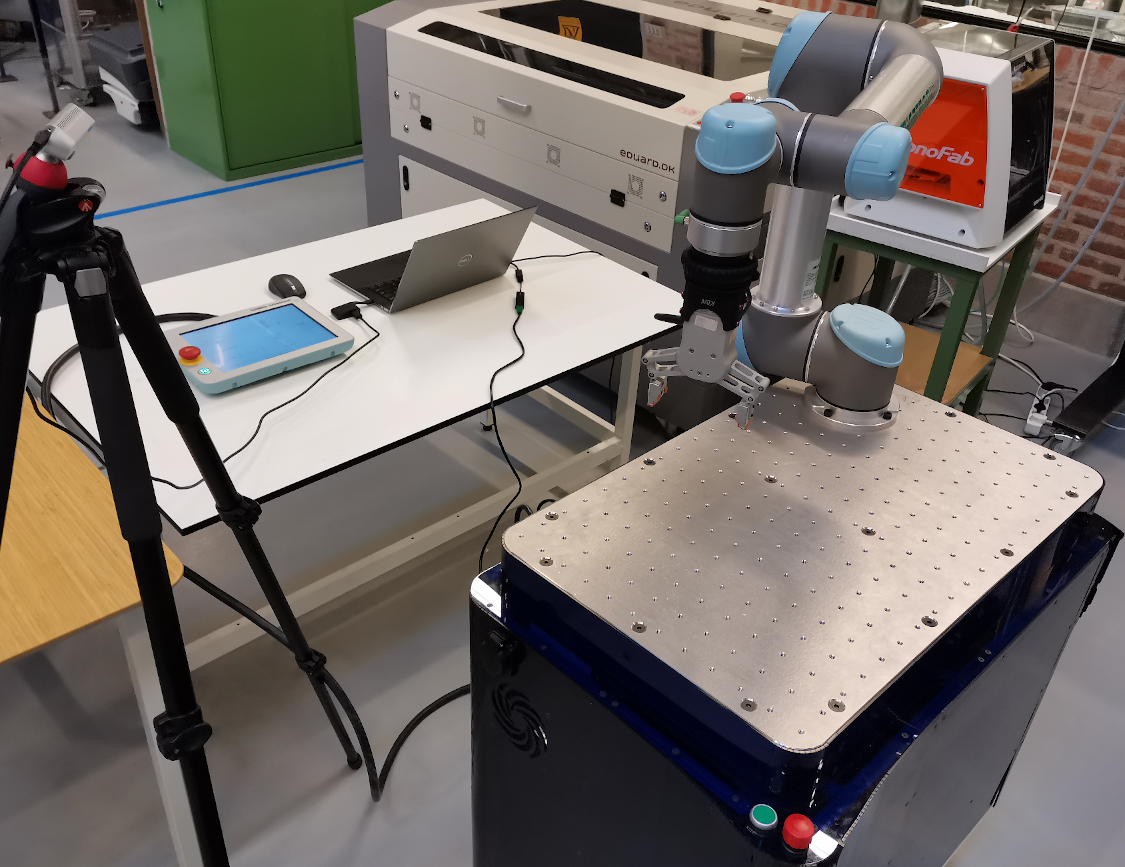
\includegraphics[width=0.75\textwidth]{experimental_evaluation/real_setup.png}
    \caption{UR5 robot with RG2 gripper and RealSense D435 camera in a setup that is used to evaluate sim-to-real transfer.}
    \label{fig:real_setup}
\end{figure}

\autoref{fig:real_objects} shows~18 different objects that were used in real world during the testing. Mostly compliant objects were selected in order to reduce the risk of damage to the gripper due to the unpredictability of end-to-end RL policy trained in a different domain. The same workspace volume and number of objects are used as in the simulation. Similarly, the goal of the agent is to lift an object within~100 time steps.

\begin{figure}[ht]
    \centering
    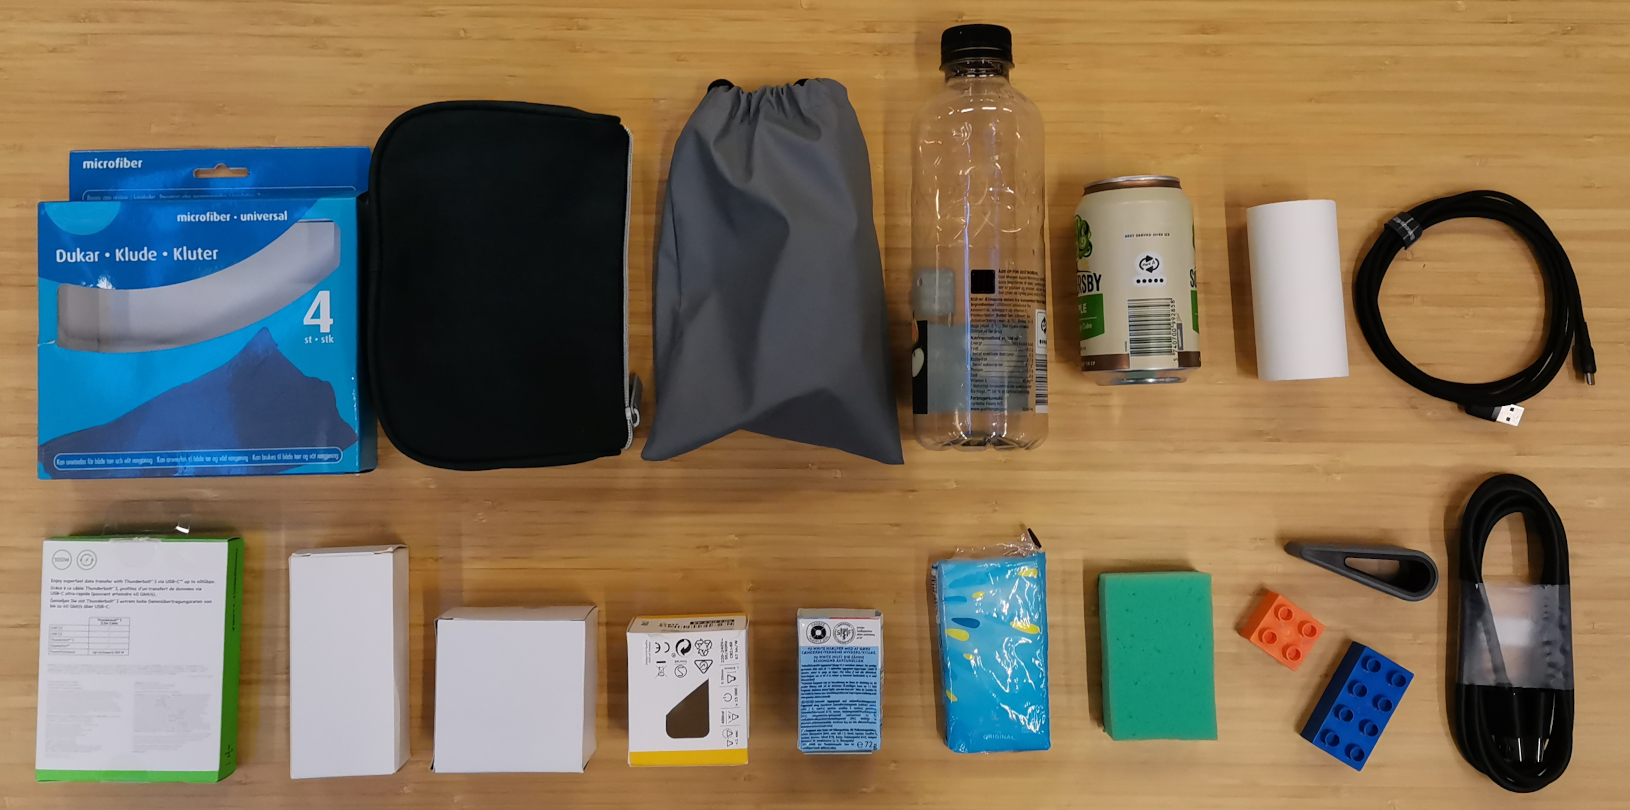
\includegraphics[width=0.75\textwidth]{experimental_evaluation/real_objects.png}
    \caption{A set of 18 objects that were used during the evaluation of sim-to-real transfer.}
    \label{fig:real_objects}
\end{figure}


\section{Results}

Results of the following experiments are presented in this section. First, actor-critic algorithms are compared on the created simulation environment in order to select the best performing one for the task of robotic grasping. Hereafter, octree-based 3D observations are compared to traditional 2D and 2.5D image observations, and studied with respect to camera pose invariance. Similarly, invariance to the utilised robot is evaluated for both training process and transfer of already learned policy. Lastly, results of sim-to-real transfer are presented.

All agents were trained over the duration of~500,000 time steps, which is assumed to provide a comparative analysis among the different experiments from this work. It is however expected, that the final performance for many of these agents can be improved with a longer training duration. On average, each agent takes three days to train from the beginning until the set duration is reached. Therefore, only a single random seed is employed for all agents due to the time-consuming training procedure and time constraints, however, use of several different seeds is encouraged as it would provide more definitive results. During evaluation of agents on novel scenes inside simulation,~200 episodes are used for each agent.


\subsection{Comparison of Actor-Critic Algorithms}

TD3, SAC and TQC were trained using the same grasping environment with a network architecture presented in \autoref{subsec:actor_critic_network_architecture} and hyperparameters from \hyperref[app:hyperparameters]{appendix~\ref*{app:hyperparameters}}. The success rate during training and the final success rate on novel objects and textures is presented in \autoref{fig:training_curve_comparison_actor_critic_algorithms} for all three algorithms.

\begin{figure}[ht]
    \centering
    % \includegraphics[width=0.75\textwidth]{experimental_evaluation/.pdf}
    \caption{Success rate of TD3, SAC and TQC algorithms on the created grasping environment.}
    \label{fig:training_curve_comparison_actor_critic_algorithms}
\end{figure}

Based on these results, TQC is utilised for all subsequent experiments.


\subsection{Comparison of 2D/2.5D/3D Observations}\label{subsec:comparison_of_2d_2_5d_3d_observations}

3D octree observations are now compared to more traditional 2D RGB and 2.5D RGB-D observations. Besides the success rate, this comparison also includes computational complexity in terms of memory usage and processing time. For octrees, feature extractor from \autoref{subsec:feature_extraction} is used. For RGB and RGB-D images, an analogous CNN feature extractor described in \hyperref[app:feature_extraction_from_rgb_and_rgbd_observations]{appendix~\ref*{app:feature_extraction_from_rgb_and_rgbd_observations}} is employed instead.  In order to make the comparison fair, the same architecture design is used with approximately the same number of learnable parameters as listed in \autoref{tab:feature_extractor_number_of_learnable_parameters_comparison}. TQC hyperparameters from \hyperref[app:hyperparameters]{appendix~\ref*{app:hyperparameters}} are used for all agents. In order to utilise the same replay buffer size for all three agents, the resolution of RGB images and depth maps had to be reduced to~128\({\times}\)128~px for all observation types, including octrees. Note that the change of image resolution does not impact the number of learnable parameters for octrees.

\begin{table}[ht]
    \centering
    \begin{tabular}{l|ccc}
                                               &
        \textbf{\begin{tabular}[c]{@{}c@{}}2D\\ RGB Image\end{tabular}} & \textbf{\begin{tabular}[c]{@{}c@{}}2.5D\\ RGB-D Image\end{tabular}} & \textbf{\begin{tabular}[c]{@{}c@{}}3D\\ Octree\end{tabular}}           \\ \hline
        Learnable Parameters                   & 229,248                                & 229,680                                & 226,494
    \end{tabular}
    \caption{Number of learnable parameters per each observation stack for the utilised RGB, RGB-D and octree-based feature extractors.}
    \label{tab:feature_extractor_number_of_learnable_parameters_comparison}
\end{table}

The three different feature extractors are first trained in the fully randomised environment. However, as results in \autoref{fig:training_curve_comparison_2d_2_5d_3d_random_camera_pose} indicate, 2D and 2.5D observations are unable to provide invariance to camera pose.

\begin{figure}[ht]
    \centering
    % \includegraphics[width=0.75\textwidth]{experimental_evaluation/.pdf}
    \caption{Success rate of RGB, RGB-D and octree-based feature extractors on environment with randomised camera pose.}
    \label{fig:training_curve_comparison_2d_2_5d_3d_random_camera_pose}
\end{figure}

Therefore, this experiment is repeated for an environment where the camera pose is static and remains unchanged throughout the entire training and subsequent evaluation on novel scenes. \autoref{fig:training_curve_comparison_2d_2_5d_3d_fixed_camera_pose} provides results for such environment with reduced domain randomisation.

\begin{figure}[ht]
    \centering
    % \includegraphics[width=0.75\textwidth]{experimental_evaluation/.pdf}
    \caption{Success rate of RGB, RGB-D and octree-based feature extractors on environment with a fixed camera pose.}
    \label{fig:training_curve_comparison_2d_2_5d_3d_fixed_camera_pose}
\end{figure}

Lastly, comparison of memory usage and computational time is presented in \autoref{tab:feature_extractor_memory_and_computational_time}.

\begin{table}[ht]
    \centering
    \begin{tabular}{r|ccc}
                                                      &
        \textbf{\begin{tabular}[c]{@{}c@{}}2D\\ RGB Image\end{tabular}}        & \textbf{\begin{tabular}[c]{@{}c@{}}2.5D\\ RGB-D Image\end{tabular}} & \textbf{\begin{tabular}[c]{@{}c@{}}3D\\ Octree\end{tabular}}                 \\ \hline
        \multirow{2}{*}{Size \textit{(per sample)}}   & \multirow{2}{*}{X}                      & \multirow{2}{*}{XX}                     & XXX (average) \\
                                                      &                                         &                                         & XXX (maximum) \\ \hline
        Pre-processing \textit{(average, per sample)} & ---                                     & ---                                     & X             \\
        Forward \textit{(average, per sample)}        & X                                       & X                                       & X             \\
        Forward \textit{(average, batch of 32)}       & X                                       & X                                       & X             \\
        Update \textit{(average, batch of 32)}        & X                                       & X                                       & X
    \end{tabular}
    \caption{Comparison of computational complexity for RGB, RGB-D and octree-based observations with their corresponding feature extractors. Pre-processing is performed during data collection and consists of point cloud processing, estimation of normals and creation of octree.}
    \label{tab:feature_extractor_memory_and_computational_time}
\end{table}


\subsection{Invariance to Camera Pose}

Based on the results of the previous experiment, agent with octree observations and fully randomised camera pose is evaluated with respect to its learned generalisation to different camera poses on novel scenes. A total of X various poses with different azimuth and height are evaluated, with corresponding results shown in \autoref{fig:invariance_to_camera_pose}.

\begin{figure}[ht]
    \centering
    % \includegraphics[width=0.75\textwidth]{experimental_evaluation/.pdf}
    \caption{Success rate to novel scenes for different camera poses.}
    \label{fig:invariance_to_camera_pose}
\end{figure}


\subsection{Invariance to Robot}

In addition to training agents with octree observations on UR5 robot with RG2 gripper, an agent is also trained on Panda robot in order to study the robustness of state-of-the-art actor-critic algorithm with octree observations to different kinematic chains and gripper designs. Comparison of success rate between UR5 and Panda can be seen in \autoref{fig:invariance_to_robot}.

% Consider skipping this figure if section gets too crowded
\begin{figure}[ht]
    \centering
    % \includegraphics[width=0.75\textwidth]{experimental_evaluation/.pdf}
    \caption{Success rate of UR5 and Panda robots using the same environment, algorithm and hyperparameters.}
    \label{fig:invariance_to_robot}
\end{figure}

Furthermore, feasibility of transferring a policy trained on one robot to another is investigated. Such transfer is evaluated on novel scenes with a policy trained on both UR5 and Panda. Results for this experiment can be found in \autoref{tab:results_robot_transfer}.

\begin{table}[ht]
    \centering
    \begin{tabular}{cr|cc}
                                                        &                & \multicolumn{2}{c}{During Evaluation}                  \\
                                                        &                & \textbf{UR5}                          & \textbf{Panda} \\ \hline
        \multirow{2}{*}{\begin{tabular}[c]{@{}c@{}}During\\ Training\end{tabular}} & \textbf{UR5}   & UR5/UR5                               & UR5/Panda      \\
                                                        & \textbf{Panda} & Panda/UR5                             & Panda/Panda
    \end{tabular}
    \caption{Comparison of success rate on novel scenes for policies trained one robot and evaluated on another. UR5 robot with RG2 gripper and Panda robot with its default gripper were evaluated.}
    \label{tab:results_robot_transfer}
\end{table}


\subsection{Sim-to-Real Transfer}

Finally, an agent trained inside simulation is evaluated in real-world domain to study the feasibility of sim-to-real transfer for environment with extensive domain randomisation and octree-based observations. Setup described in \autoref{subsec:real_setup} is used, where objects are randomly replaced after each success or~100 time steps. With this setup,~41 out of~60 episodes were successful, which results in a success rate of~68\%. \autoref{fig:sim_to_real_success_examples} shows few examples of successful grasps and a recording is available on YouTube\footnote{\href{https://youtube.com/watch?v=btxqzFOgCyQ&list=PLzcIGFRbGF3Qr4XSzAjNwOMPaeDn5J6i1}{https://youtube.com/watch?v=btxqzFOgCyQ}}.

\begin{figure}[ht]
    \centering
    % \includegraphics[width=0.75\textwidth]{experimental_evaluation/.pdf}
    \caption{Examples of successful grasps accomplished by a policy that was transferred from simulation to real-world domain.}
    \label{fig:sim_to_real_success_examples}
\end{figure}


\section{Ablation Studies}

Besides results presented in the previous section, various ablations of the full approach are studied in order to determine contributions of its components. It is believed that these results are applicable also for other robotics tasks that utilise visual observations. \autoref{fig:ablation_studies} presents these ablations with respect to their learning curve and attainable success rate.

\begin{figure}[ht]
    \centering
    % \includegraphics[width=0.75\textwidth]{experimental_evaluation/.pdf}
    \caption{Success rate of various ablations of the full method with octree observations.}
    \label{fig:ablation_studies}
\end{figure}

\paragraph{Demonstrations} Preloading experience replay buffer with demonstrations ...

\paragraph{Curriculum} Similar to demonstrations, curriculum is meant to ...

\paragraph{Colour Features} By removing colour features from the octree ...
"When comparing agents with and without colour features, an agent with colour features is more successful at grasping small objects."


\paragraph{Proprioceptive Observations} Addition of proprioceptive observations has ...

\paragraph{Sharing of Feature Extractor between Actor and Critics} Using a shared feature extractor for actor and critic ...

\paragraph{Separate Feature Extractors for Stacked Observations} If a shared feature extractor is used for all stacked observations, ...
